%%%%%%%%%%%%%%%%%%%%%%%%%%%%%%%%%%%%%%%%%%%%%%%%%%%%%%%%%
%%%%%%%%%%%%%%%%%%%%%%%%%%%%%%%%%%%%%%%%%%%%%%%%%%%%%%%%%
\section{The Problem:}
\subsection{Qualitative Diagnosis and Prognosis}
%%%%%%%%%%%%%%%%%%%%%%%%%%%%%%%%%%%%%%%%%%%%%%%%%%%%%%%%%
%%%%%%%%%%%%%%%%%%%%%%%%%%%%%%%%%%%%%%%%%%%%%%%%%%%%%%%%%



%%%%%%%%%%%%%%%%%%%%%%%%%%%%%%%%%%%%%%%%%%%%%%%%%%%%%%%%%
\begin{frame}
\frametitle{Prostate Cancer}
\framesubtitle{The Question is \emph{Will He Outlive It?}}


    \begin{block}{}
        \begin{itemize}
            \item More than $225,000$ cases per year (USA).
            \item One is seven men will be diagnosed.
            \item Treatments: surgery, chemo, radiation, harmone therapy.
            \item Either slowly-growing  and benign or fast-growing
                and dangerous.
            \item Surgery / radiation benefits questionable for SG/B.
            \item Surgery / radiation side effects not desirable.
            \item ... therefore, active surveillance.
        \end{itemize}
    \end{block}

\end{frame}
%%%%%%%%%%%%%%%%%%%%%%%%%%%%%%%%%%%%%%%%%%%%%%%%%%%%%%%%%

%%%%%%%%%%%%%%%%%%%%%%%%%%%%%%%%%%%%%%%%%%%%%%%%%%%%%%%%%
\begin{frame}
\frametitle{Prostate Cancer}
\framesubtitle{Diagnosis}

\centering
    \only<1>{
\includegraphics[width=\textwidth]{../FIGS/gleason/gleason-process-1}}%
    \only<2>{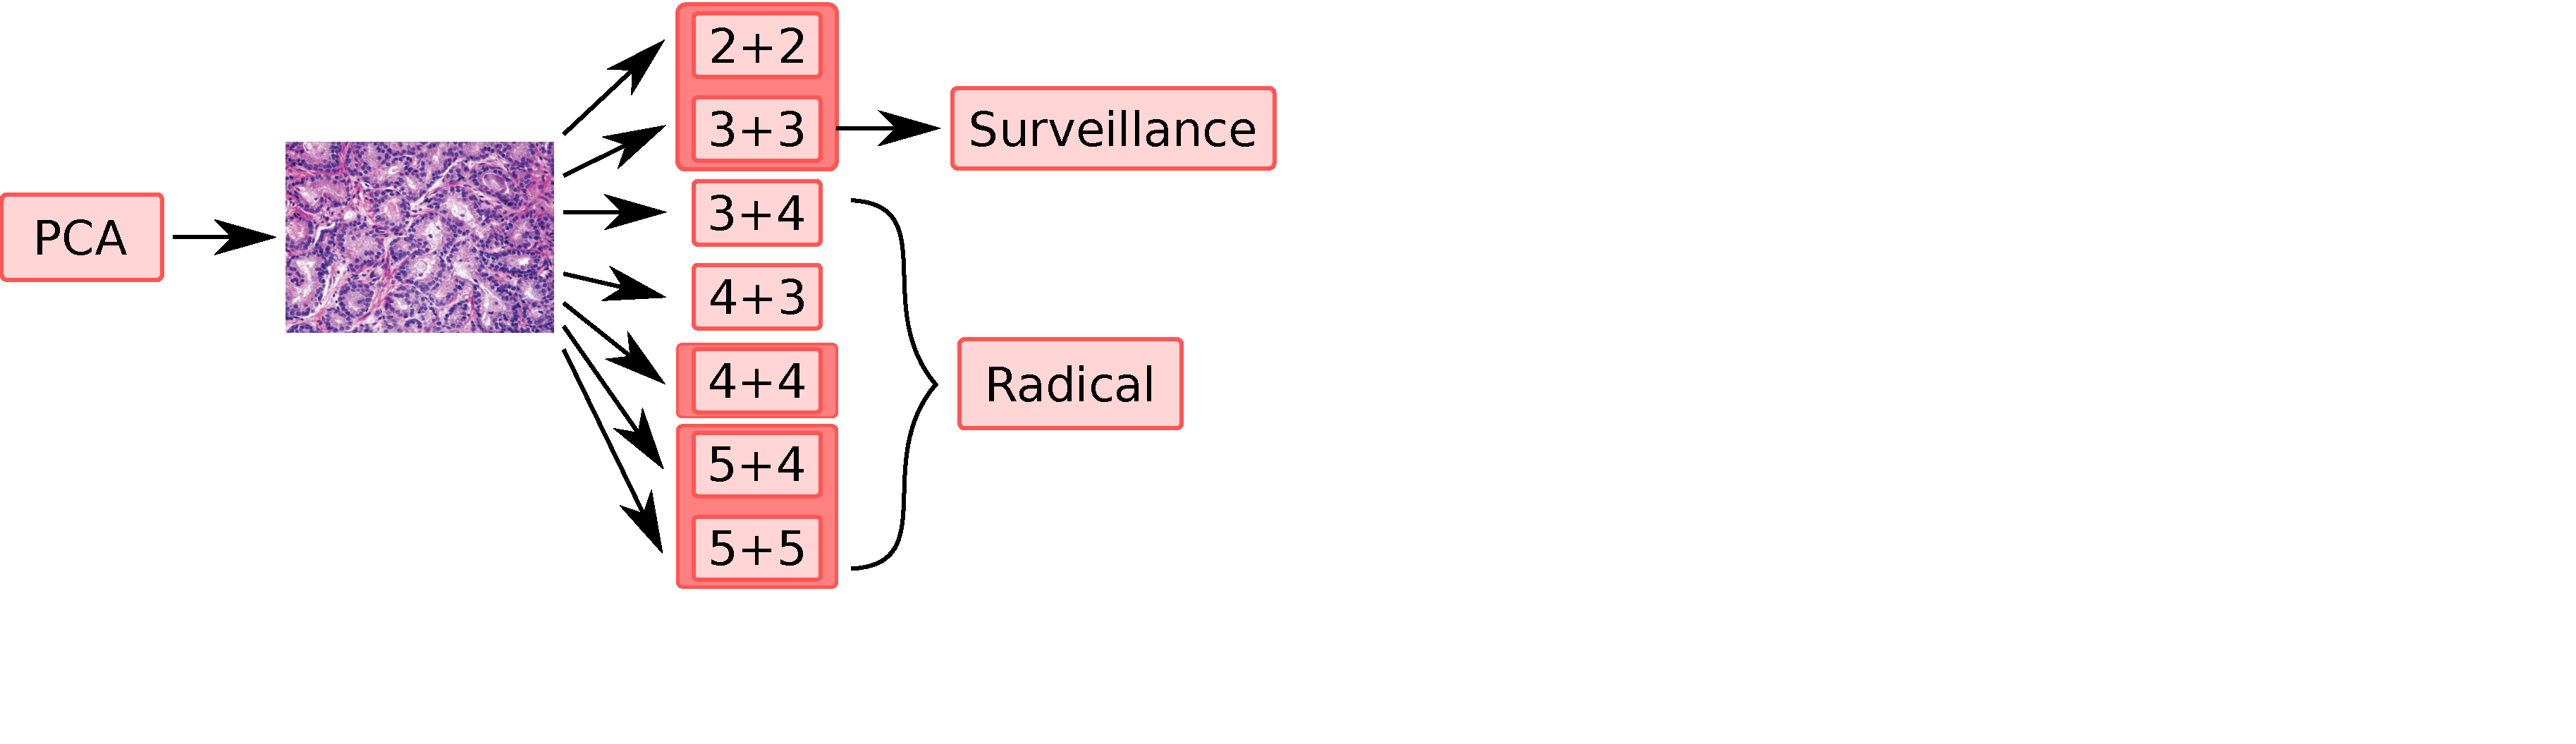
\includegraphics[width=\textwidth]{../FIGS/gleason/gleason-process-2}}%
    \only<3>{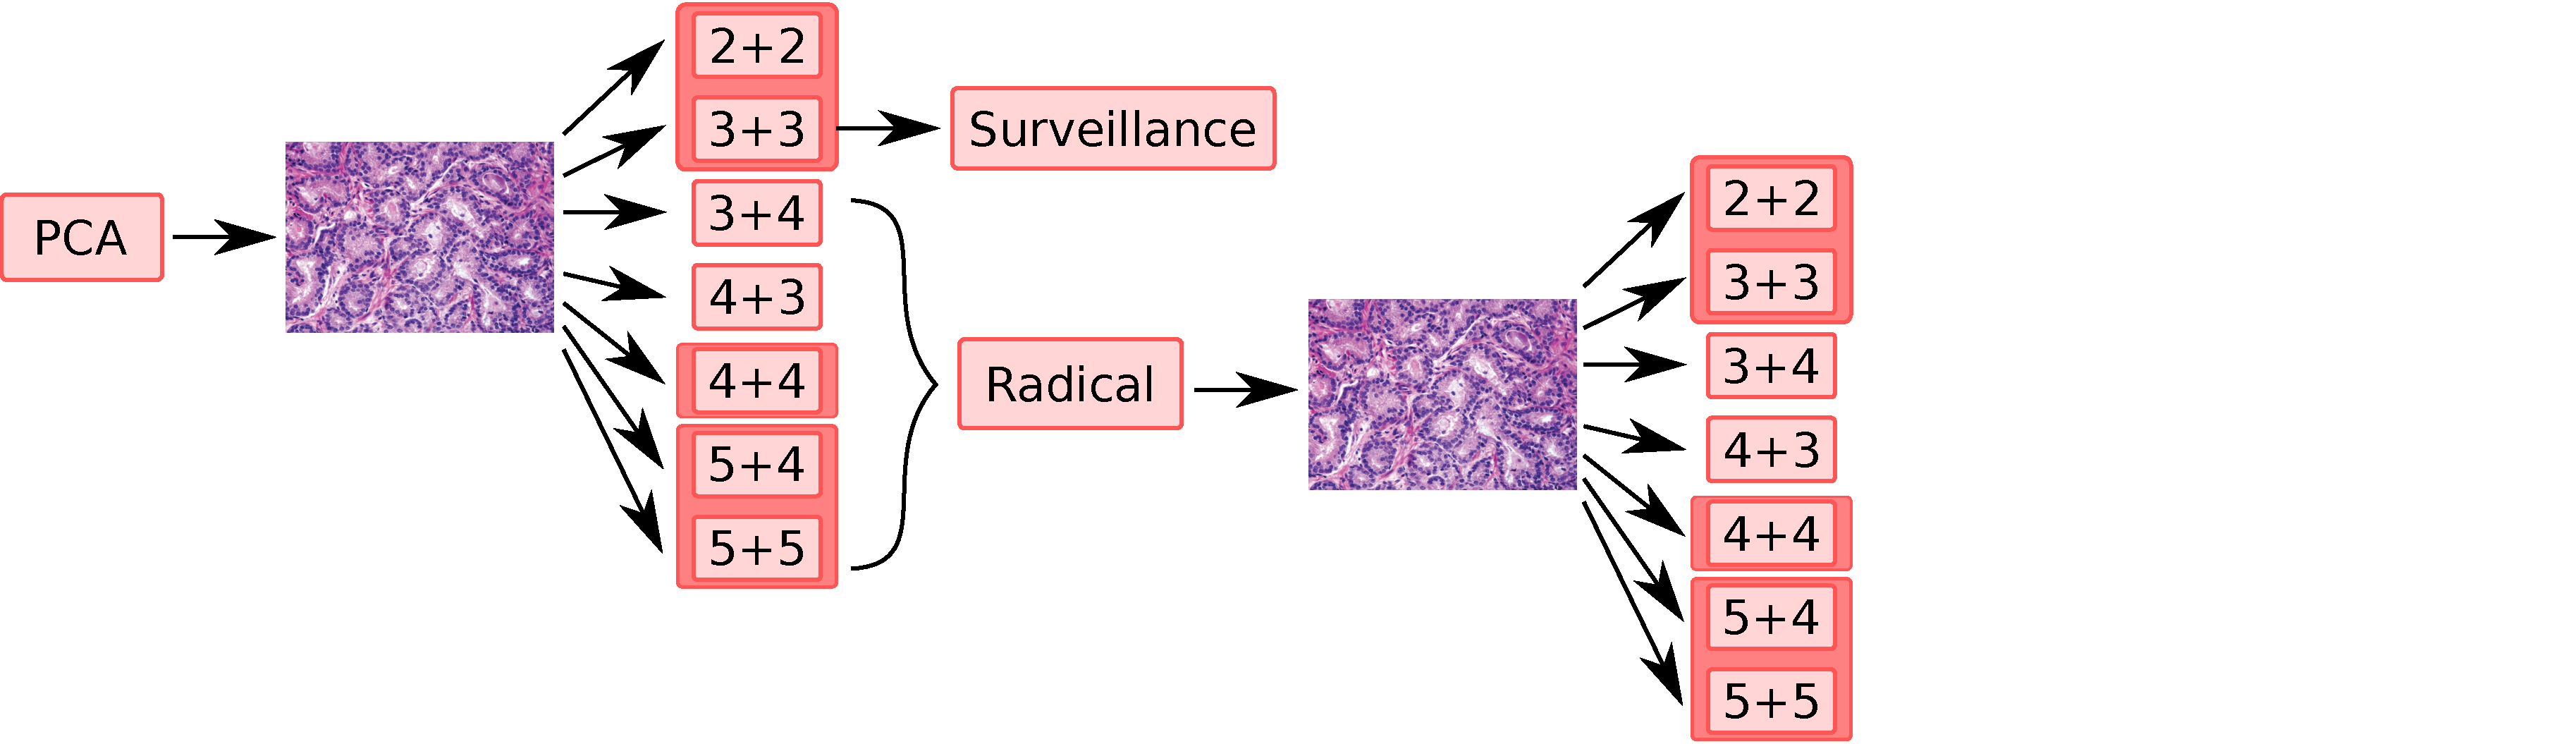
\includegraphics[width=\textwidth]{../FIGS/gleason/gleason-process-3}}%
    \only<4->{\includegraphics[width=\textwidth]{../FIGS/gleason/gleason-process}}

\end{frame}
%%%%%%%%%%%%%%%%%%%%%%%%%%%%%%%%%%%%%%%%%%%%%%%%%%%%%%%%%


%%%%%%%%%%%%%%%%%%%%%%%%%%%%%%%%%%%%%%%%%%%%%%%%%%%%%%%%%
\begin{frame}
\frametitle{Biopsy and Prostectmy Slides}
\framesubtitle{How to Describe Glandular Architecture}

        \centering
        \only<1->{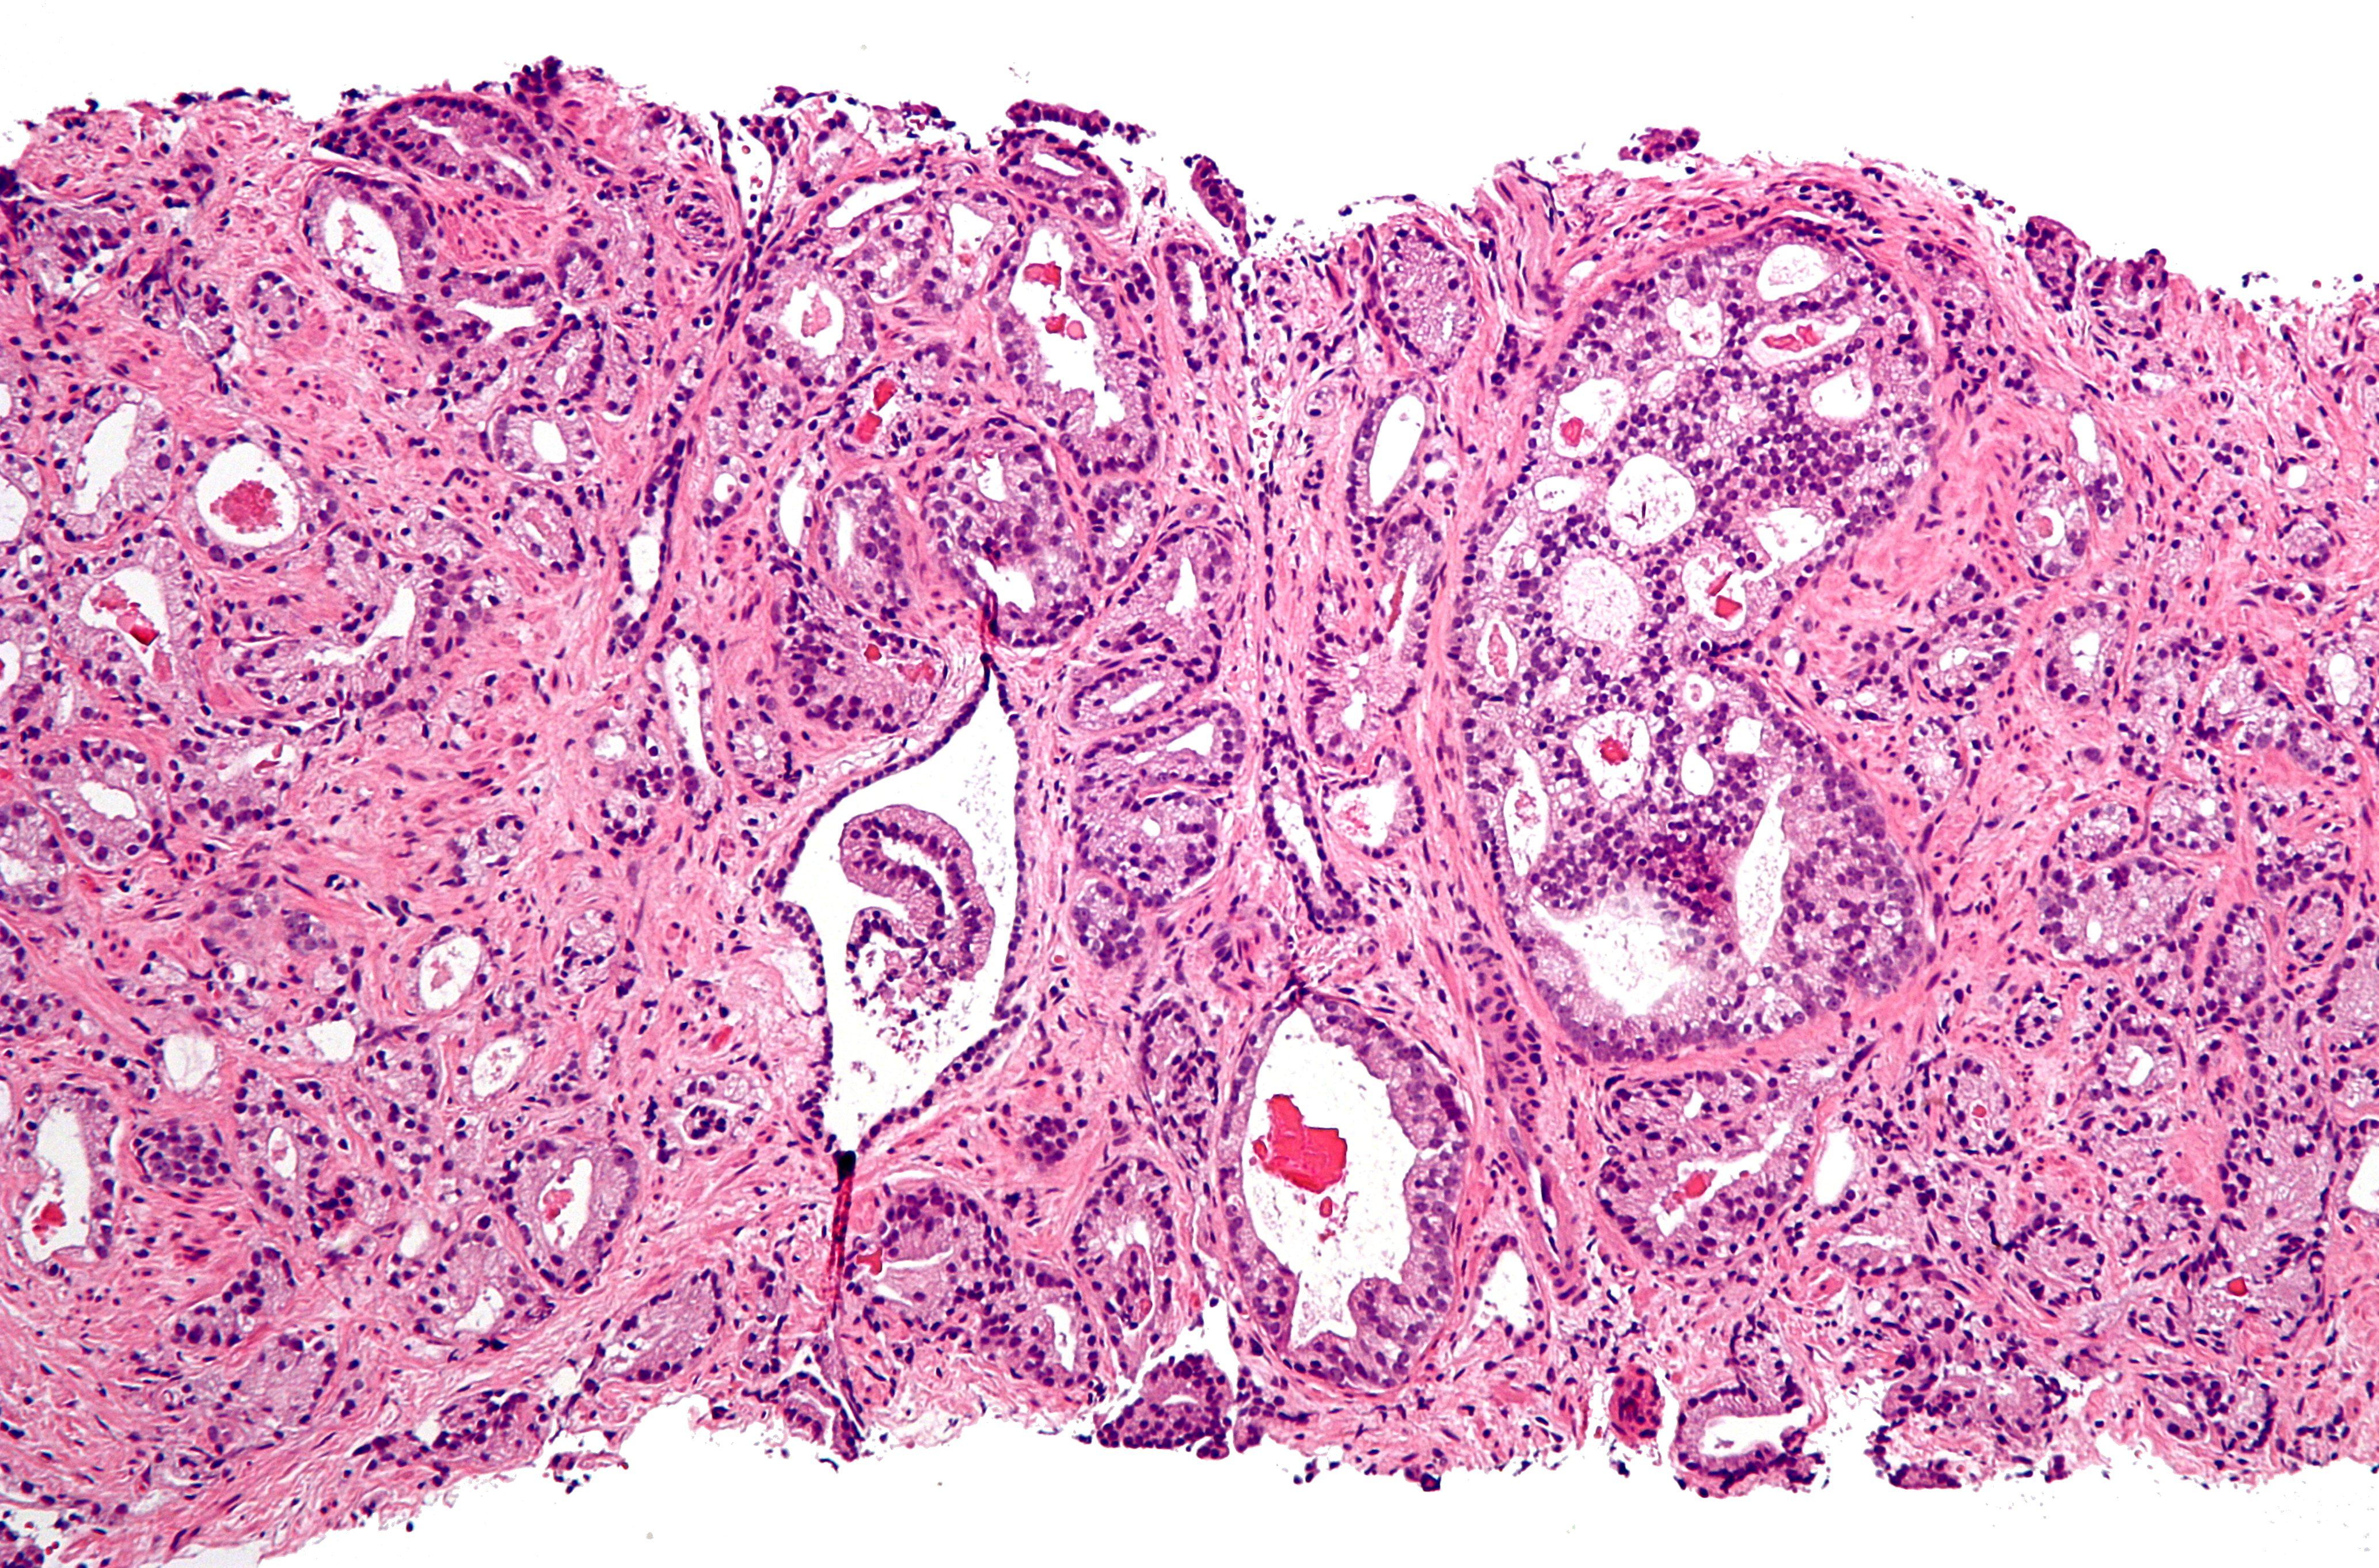
\includegraphics[height=2.5in]{gleason-4}}

\end{frame}
%%%%%%%%%%%%%%%%%%%%%%%%%%%%%%%%%%%%%%%%%%%%%%%%%%%%%%%%%


%%%%%%%%%%%%%%%%%%%%%%%%%%%%%%%%%%%%%%%%%%%%%%%%%%%%%%%%%
\begin{frame}
\frametitle{Gleason Grading}
\framesubtitle{~}

    \begin{columns}
        \column{.45\textwidth}
        \centering
        \only<1>{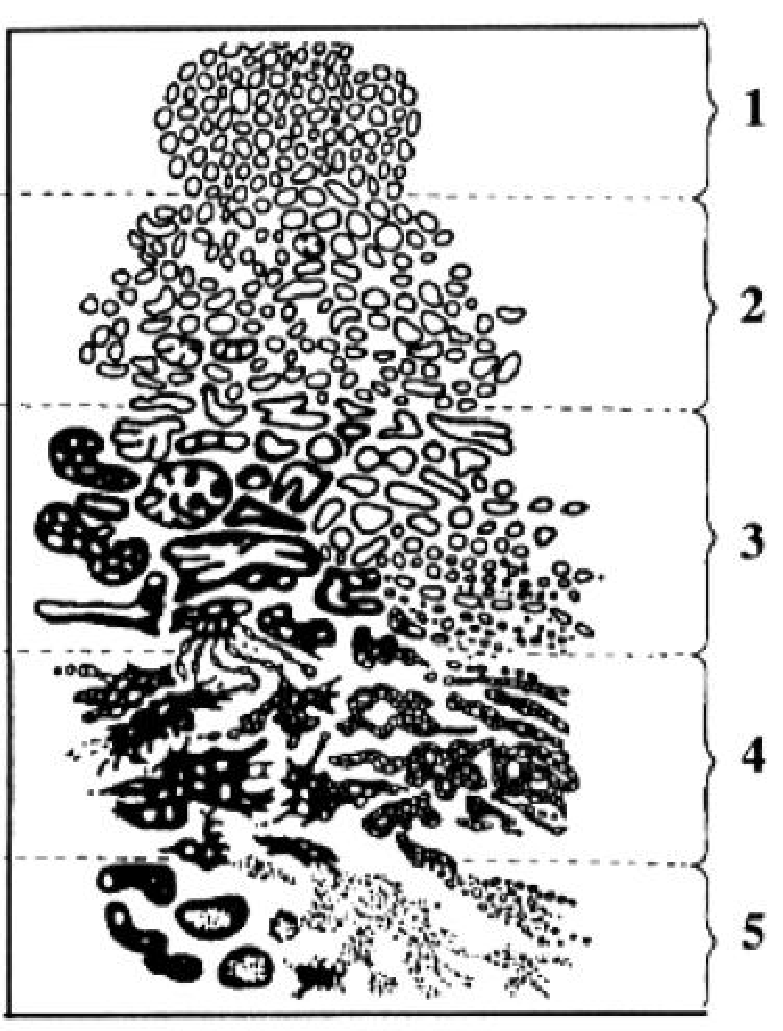
\includegraphics[height=2in]{../FIGS/gleason/gleason}}
        \only<2->{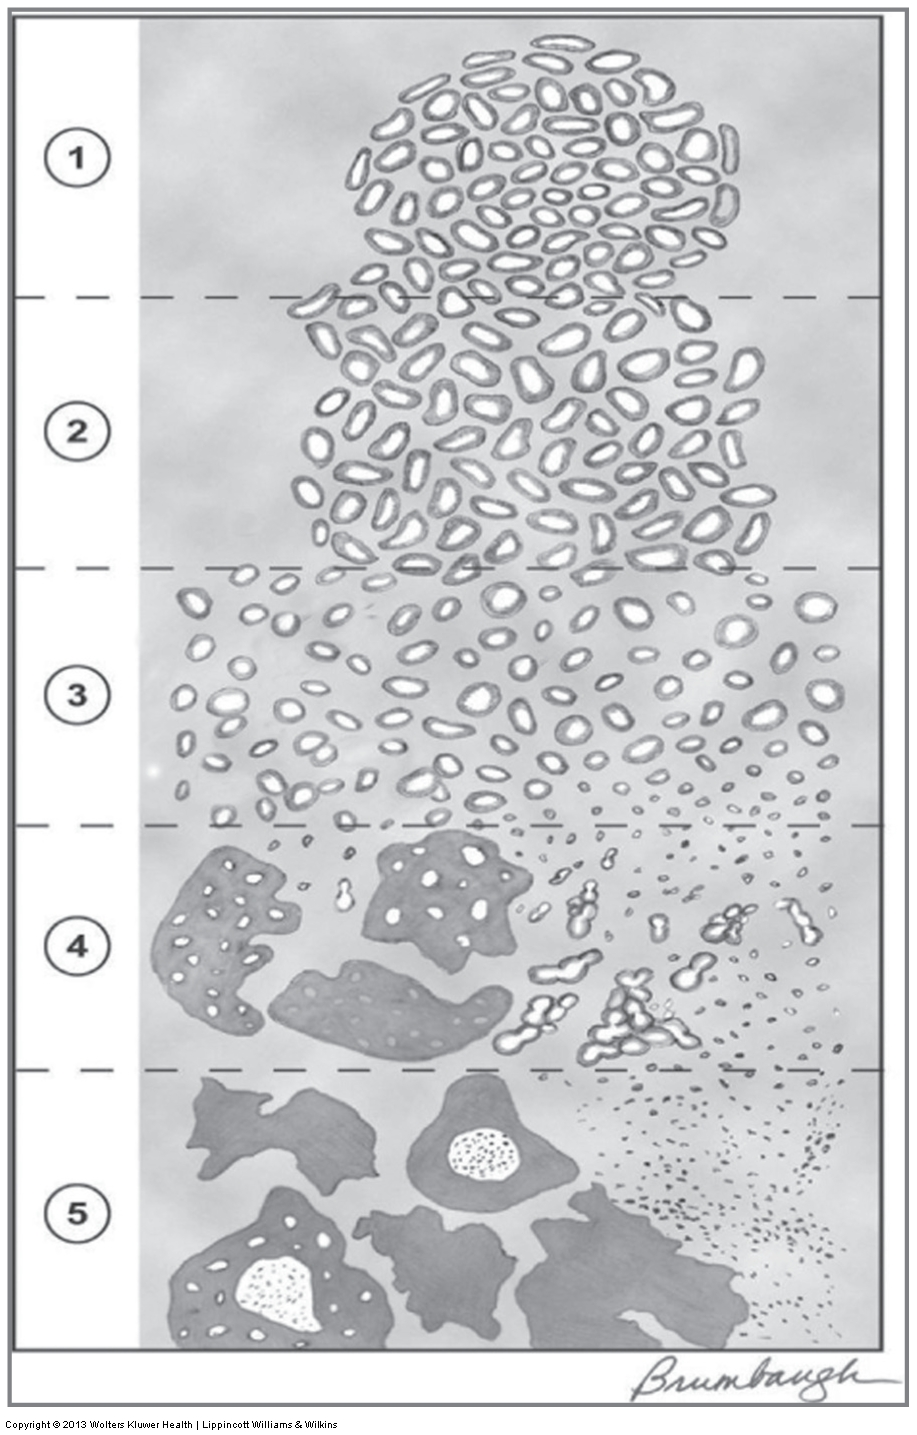
\includegraphics[height=2in]{../FIGS/gleason/epp-figure_1-4}}
        \column{.45\textwidth}
        \begin{block}{}
            \hangindent=1.5cm
            \hangafter=1
            \noindent
            Grade 1: well-defined, nicely packed
             
            \hangindent=1.5cm
            \hangafter=1
            \noindent
            Grade 2: larger, more tissue,  less uniform
        

            \hangindent=1.5cm
            \hangafter=1
            \noindent
            Grade 3: less defined glands% 
            \only<1>{, some cribriform}
            
            \hangindent=1.5cm
            \hangafter=1
            \noindent
            Grade 4: fused glands, open lumens%
            \only<2->{, cribriform}

            \hangindent=1.5cm
            \hangafter=1
            \noindent
            Grade 5: no glandular definition, sheets of cells
        \end{block}
    \end{columns}
    \only<1>{\footnotetext{
        Donald Gleason, 1966, image from \emph{The Gleason Grading System: A Complete
        Guide for Pathologist and Clinicians} by Eppstein}}
    \only<2>{\footnotetext{
        2005 Consensus, image from \emph{The Gleason Grading System: A Complete
        Guide for Pathologist and Clinicians} by Eppstein}}

\end{frame}
%%%%%%%%%%%%%%%%%%%%%%%%%%%%%%%%%%%%%%%%%%%%%%%%%%%%%%%%%

%%%%%%%%%%%%%%%%%%%%%%%%%%%%%%%%%%%%%%%%%%%%%%%%%%%%%%%%%
\begin{frame}
    \frametitle{Learning to Grade}
    \framesubtitle{\emph{The Gleason Grading System: A Complete Guide for
    Pathologists and Clinicians}}

    \centering
    
\includegraphics[height=3in]{gleason-book}

\end{frame}
%%%%%%%%%%%%%%%%%%%%%%%%%%%%%%%%%%%%%%%%%%%%%%%%%%%%%%%%%


%%%%%%%%%%%%%%%%%%%%%%%%%%%%%%%%%%%%%%%%%%%%%%%%%%%%%%%%%
\begin{frame}
\frametitle{Glandular Architecture}
    \framesubtitle{Discrete-vs-Fused Glands}

    \begin{columns}
        \column{.45\textwidth}
        \centering
        \includegraphics[width=\textwidth]{figure_2-284_fused}
        \column{.45\textwidth}
        \begin{block}{Gleason 3}
            Discrete glands. 
        \end{block}
        \begin{block}{Gleason 4}
            Presence of fused glands. 
        \end{block}
    \end{columns}
    \only<1->{\footnotetext{Image source: Eppstein, \emph{The Gleason Grading
  System}}}
    
\end{frame}
%%%%%%%%%%%%%%%%%%%%%%%%%%%%%%%%%%%%%%%%%%%%%%%%%%%%%%%%%

%%%%%%%%%%%%%%%%%%%%%%%%%%%%%%%%%%%%%%%%%%%%%%%%%%%%%%%%%
\begin{frame}
\frametitle{Glandular Architecture}
    \framesubtitle{Cribriform Pattern}

    \begin{columns}
        \column{.45\textwidth}
        \centering
        \includegraphics[width=\textwidth]{figure_2-133-cribriform}
        \column{.45\textwidth}
        \begin{block}{Gleason 4}
            {A gland with numerous small~holes.}
        \end{block}
    \end{columns}
    \only<1->{\footnotetext{Image source: Eppstein, \emph{The Gleason Grading
    System}}}

\end{frame}
%%%%%%%%%%%%%%%%%%%%%%%%%%%%%%%%%%%%%%%%%%%%%%%%%%%%%%%%%

%%%%%%%%%%%%%%%%%%%%%%%%%%%%%%%%%%%%%%%%%%%%%%%%%%%%%%%%%
\begin{frame}
\frametitle{Glandular Architecture}
    \framesubtitle{Glomeruloid Structures}

    \begin{columns}
        \column{.45\textwidth}
        \centering
        \includegraphics[width=\textwidth]{glomeroid}
        \column{.45\textwidth}
        \begin{block}{Gleason 3,4}
            Intraluminal cribriform, single point of attachment.
        \end{block}
    \end{columns}
    \only<1->{\footnotetext{Image source: 
    \url{http://www.nature.com/modpathol/journal/v17/n3/fig_tab/3800050f9.html}
    }}

\end{frame}
%%%%%%%%%%%%%%%%%%%%%%%%%%%%%%%%%%%%%%%%%%%%%%%%%%%%%%%%%


%%%%%%%%%%%%%%%%%%%%%%%%%%%%%%%%%%%%%%%%%%%%%%%%%%%%%%%%%
\begin{frame}
\frametitle{Glandular Architecture}
    \framesubtitle{Telescoping Glands}

    \begin{columns}
        \column{.45\textwidth}
        \centering
        \includegraphics[width=\textwidth]{figure_2-215_telescoping}
        \column{.45\textwidth}
        \begin{block}{Gleason 3}
            Telescoping (gland in gland) may mimic Glumeroid. 
        \end{block}
        \begin{block}{Gleason 4}
            Actual glumeroid pattern. 
        \end{block}
    \end{columns}
    \only<1->{\footnotetext{Image source: Eppstein, \emph{The Gleason Grading
    System}}}

\end{frame}
%%%%%%%%%%%%%%%%%%%%%%%%%%%%%%%%%%%%%%%%%%%%%%%%%%%%%%%%%


%%%%%%%%%%%%%%%%%%%%%%%%%%%%%%%%%%%%%%%%%%%%%%%%%%%%%%%%%
\begin{frame}
\frametitle{Glandular Architecture}
    \framesubtitle{Distribution of Glandular Shape and Size}

    \begin{columns}
        \column{.45\textwidth}
        \centering
        \includegraphics[height=1in]{gland}\\
        \includegraphics[height=1in]{figure_2-4_packed}
        \column{.45\textwidth}
        \begin{block}{Gleason 1}
            Uniform distribution of gland size. Round.
        \end{block}
        \begin{block}{Gleason 3}
            Irregularly separated glands.
        \end{block}
        \begin{block}{Gleason 4}
            Poorly formed glands.
        \end{block}
    \end{columns}
    \only<1->{\footnotetext{Image source: Eppstein, \emph{The Gleason Grading
    System}}}
\end{frame}
%%%%%%%%%%%%%%%%%%%%%%%%%%%%%%%%%%%%%%%%%%%%%%%%%%%%%%%%%


